\section{Aggregate Stats}

The EDA is bootstrapped through the following function, which is called by function \texttt{main()}:

\begin{minted}[linenos = true]{R}
eda <- function(dt) {
  plot_summary(calc_summary(dt))
  plot_seasons(determine_hemispheres(dt))
}
\end{minted}

This section focuses on the first part of the conducted EDA, which addresses aggregate statistics deduced from the dataset.
These are calculated in \texttt{calc\_summary()} and plotted (after being further processed) in \texttt{plot\_summary()}.

\begin{minted}[linenos = true, escapeinside=@@]{R}
calc_summary <- function(dt) {
  countries <- unique(dt$Country)
  aggr_dt <- function(group) {                                    @\label{aggr_dt_A}@
    dt[Country %in% group,
       .(
         total.deaths         = sum(deaths.inc),
         total.confirmed      = sum(confirmed.ind),
         total.ratio          = sum(deaths.inc) / sum(confirmed.ind),
         mean.daily.confirmed = mean(confirmed.ind),
         mean.daily.deaths    = mean(deaths.inc)
        ),
       by = .(Country)]
  }                                                               @\label{aggr_dt_Z}@
  all_agdt <- aggr_dt(countries)
  mean_dt <- function(name, group) {                              @\label{mean_dt_A}@
    all_agdt[Country %in% group,
             .(
               Country              = name,
               total.deaths         = sum(total.deaths),
               total.confirmed      = sum(total.confirmed),
               total.ratio          = mean(total.ratio),
               mean.daily.confirmed = mean(mean.daily.confirmed),
               mean.daily.deaths    = mean(mean.daily.deaths)
              )]
  }                                                               @\label{mean_dt_Z}@
  world <- mean_dt("WORLD", countries)                            @\label{calc_sum_1}@
  eu    <- mean_dt("EUROPEAN UNION", EU)
  nord  <- mean_dt("NORDIC COUNTRIES", NORDIC)
  brics <- mean_dt("BRICS", BRICS)
  balk  <- mean_dt("BALKAN COUNTRIES", BALKANS)
  gulf  <- mean_dt("GULF COUNTRIES", GULF)                        @\label{calc_sum_2}@

  rbind(all_agdt, world, eu, nord, brics, balk, gulf)             @\label{calc_sum_ret}@
}
\end{minted}

Function \texttt{calc\_sum()}, using the auxiliary function \texttt{aggr\_dt} (lines \ref{aggr_dt_A}-\ref{aggr_dt_Z}) and the closure \texttt{mean\_dt} over the local variable \texttt{all\_agdt} (lines \ref{mean_dt_A}-\ref{mean_dt_Z}), calculates the aggregate statistics for some predefined geographic and economic groups of countries that would be interesting to compare (lines \ref{calc_sum_1}-\ref{calc_sum_2}), and returns them through the enrichment of the initially given \texttt{data.table} (line \ref{calc_sum_ret}).

The resulting \texttt{data.table} is piped into the \texttt{plot\_summary} function, which further transforms it to facilitate and conduct the creation of the plots.

In the following listing, lines \ref{econ_A}-\ref{econ_Z} create a temporary factor variable and two stack barplots (Figures \ref{fig:aggr_econ_conf} and \ref{fig:aggr_econ_deaths}) for the total confirmed COVID-19 cases and the total deaths attributed to the virus, respectively, for three major economic groups of countries: the European Union, the BRICS (Brazil, Russia, India, China and South Africa) and the US (which is considered as a whole separate economy here, due to both its vast size and its unique structure).

Subsequently, lines \ref{geo_A}-\ref{geo_Z} repeat a similar procedure, though this time for geographic groups: countries that are mostly or partially ($>= 25\%$ of their area) in the Balkan Peninsula according to \cite{wikibalkans}, the countries that constitute the Arab states of the Persian Gulf according to \cite{wikigulf} and the Nordic countries. 
These are presented in Figures \ref{fig:aggr_geo_conf} and \ref{fig:aggr_geo_deaths}.

\begin{minted}[linenos = true, escapeinside=@@]{R}
plot_summary <- function(dt) {
  # Stack barplots for economic groups                               @\label{econ_A}@
  econ <- dt[Country %in% c(EU, BRICS, "US")
            ][, econ.grp := as.factor(ifelse(Country %in% EU,
                                             "European Union",
                                             ifelse(Country %in% BRICS,
                                                    "BRICS",
                                                    "US")))]
  ggplot(econ) + aes(x = econ.grp, y = total.confirmed, fill = Country) +
    geom_bar(position = "stack", stat = "identity") +
    labs(title = "Confirmed COVID-19 cases per economic group") +
    labs(subtitle = "Dataset from CSSE, Johns Hopkins University") +
    labs(x = "", y = "Confirmed COVID-19 Cases") + theme_bw() +
    geom_text(aes(label = Country), position = position_stack(vjust=.5), size=2)
  ggsave("aggr_econ_conf.png")
  ggplot(econ) + aes(x = econ.grp, y = total.deaths, fill = Country) +
    geom_bar(position = "stack", stat = "identity") +
    labs(title = "COVID-19 deaths per economic group") +
    labs(subtitle = "Dataset from CSSE, Johns Hopkins University") +
    labs(x = "", y = "COVID-19 Deaths") + theme_bw() +
    geom_text(aes(label = Country), position = position_stack(vjust=.5), size=2)
  ggsave("aggr_econ_deaths.png")                                     @\label{econ_Z}@
  
  # Stack barplots for geographic groups                             @\label{geo_A}@
  geogr <- dt[Country %in% c(BALKANS, NORDIC, GULF)
             ][, geo.grp := as.factor(ifelse(Country %in% BALKANS,
                                              "Balkan",
                                              ifelse(Country %in% NORDIC,
                                                     "Nordic",
                                                     "Gulf")))]
  ggplot(geogr) + aes(x = geo.grp, y = total.confirmed, fill = Country) +
    geom_bar(position = "stack", stat = "identity") +
    labs(title = "Confirmed COVID-19 cases per geographic group") +
    labs(subtitle = "Dataset from CSSE, Johns Hopkins University") +
    labs(x = "", y = "Confirmed COVID-19 Cases") + theme_bw() +
    geom_text(aes(label = Country), position = position_stack(vjust=.5), size=2)
  ggsave("aggr_geo_conf.png")
  ggplot(geogr) + aes(x = geo.grp, y = total.deaths, fill = Country) +
    geom_bar(position = "stack", stat = "identity") +
    labs(title = "COVID-19 deaths per geographic group") +
    labs(subtitle = "Dataset from CSSE, Johns Hopkins University") +
    labs(x = "", y = "COVID-19 Deaths") + theme_bw() +
    geom_text(aes(label=Country), position=position_stack(vjust=.5), size=2)
  ggsave("aggr_geo_deaths.png")                                      @\label{geo_Z}@
  
  # Lollipop plots for death-to-confirmed ratios                     @\label{ratio_A}@
  aggrs <- c("WORLD", "EUROPEAN UNION", "NORDIC COUNTRIES", "BRICS",
             "BALKAN COUNTRIES", "GULF COUNTRIES", "US")
  bottom25 <- dt[!Country %in% c("MS Zaandam", "Diamond Princess")
                ][order(-total.ratio)][1:25]
  ratioz <- rbind(dt[Country %in% aggrs], bottom25)[order(-total.ratio)]
  ratioz$Country <- reorder(ratioz$Country, ratioz$total.ratio)
  ggplot(ratioz) + aes(x = Country, y = total.ratio) +
    geom_segment(aes(x = Country, xend = Country, y = 0, yend = total.ratio),
                 color = ifelse(ratioz$Country %in% aggrs, "blue", "dark red"),
                 size  = ifelse(ratioz$Country %in% aggrs, 1.3, 0.7) ) +
    geom_text(aes(label=sprintf("%d out of %d", total.deaths,total.confirmed)),
              vjust = .5, hjust = -.15, color="magenta", size = 1.5) +
    ylim(c(0, .31)) +
    geom_point(color = ifelse(ratioz$Country %in% aggrs, "blue", "dark red"),
               size  = ifelse(ratioz$Country %in% aggrs, 3, 1)) +
    coord_flip() + labs(x = "", y = "Ratio") + theme_bw() +
    labs(title = "Ratio of COVID-19 Deaths to Confirmed COVID-19 Cases") +
    labs(subtitle = "Dataset from CSSE, Johns Hopkins University")
  ggsave("aggr_ratio_lollipop.png")                                  @\label{ratio_Z}@
}
\end{minted}

\begin{figure}[H]
\centering
\begin{minipage}{.5\textwidth}
  \centering
  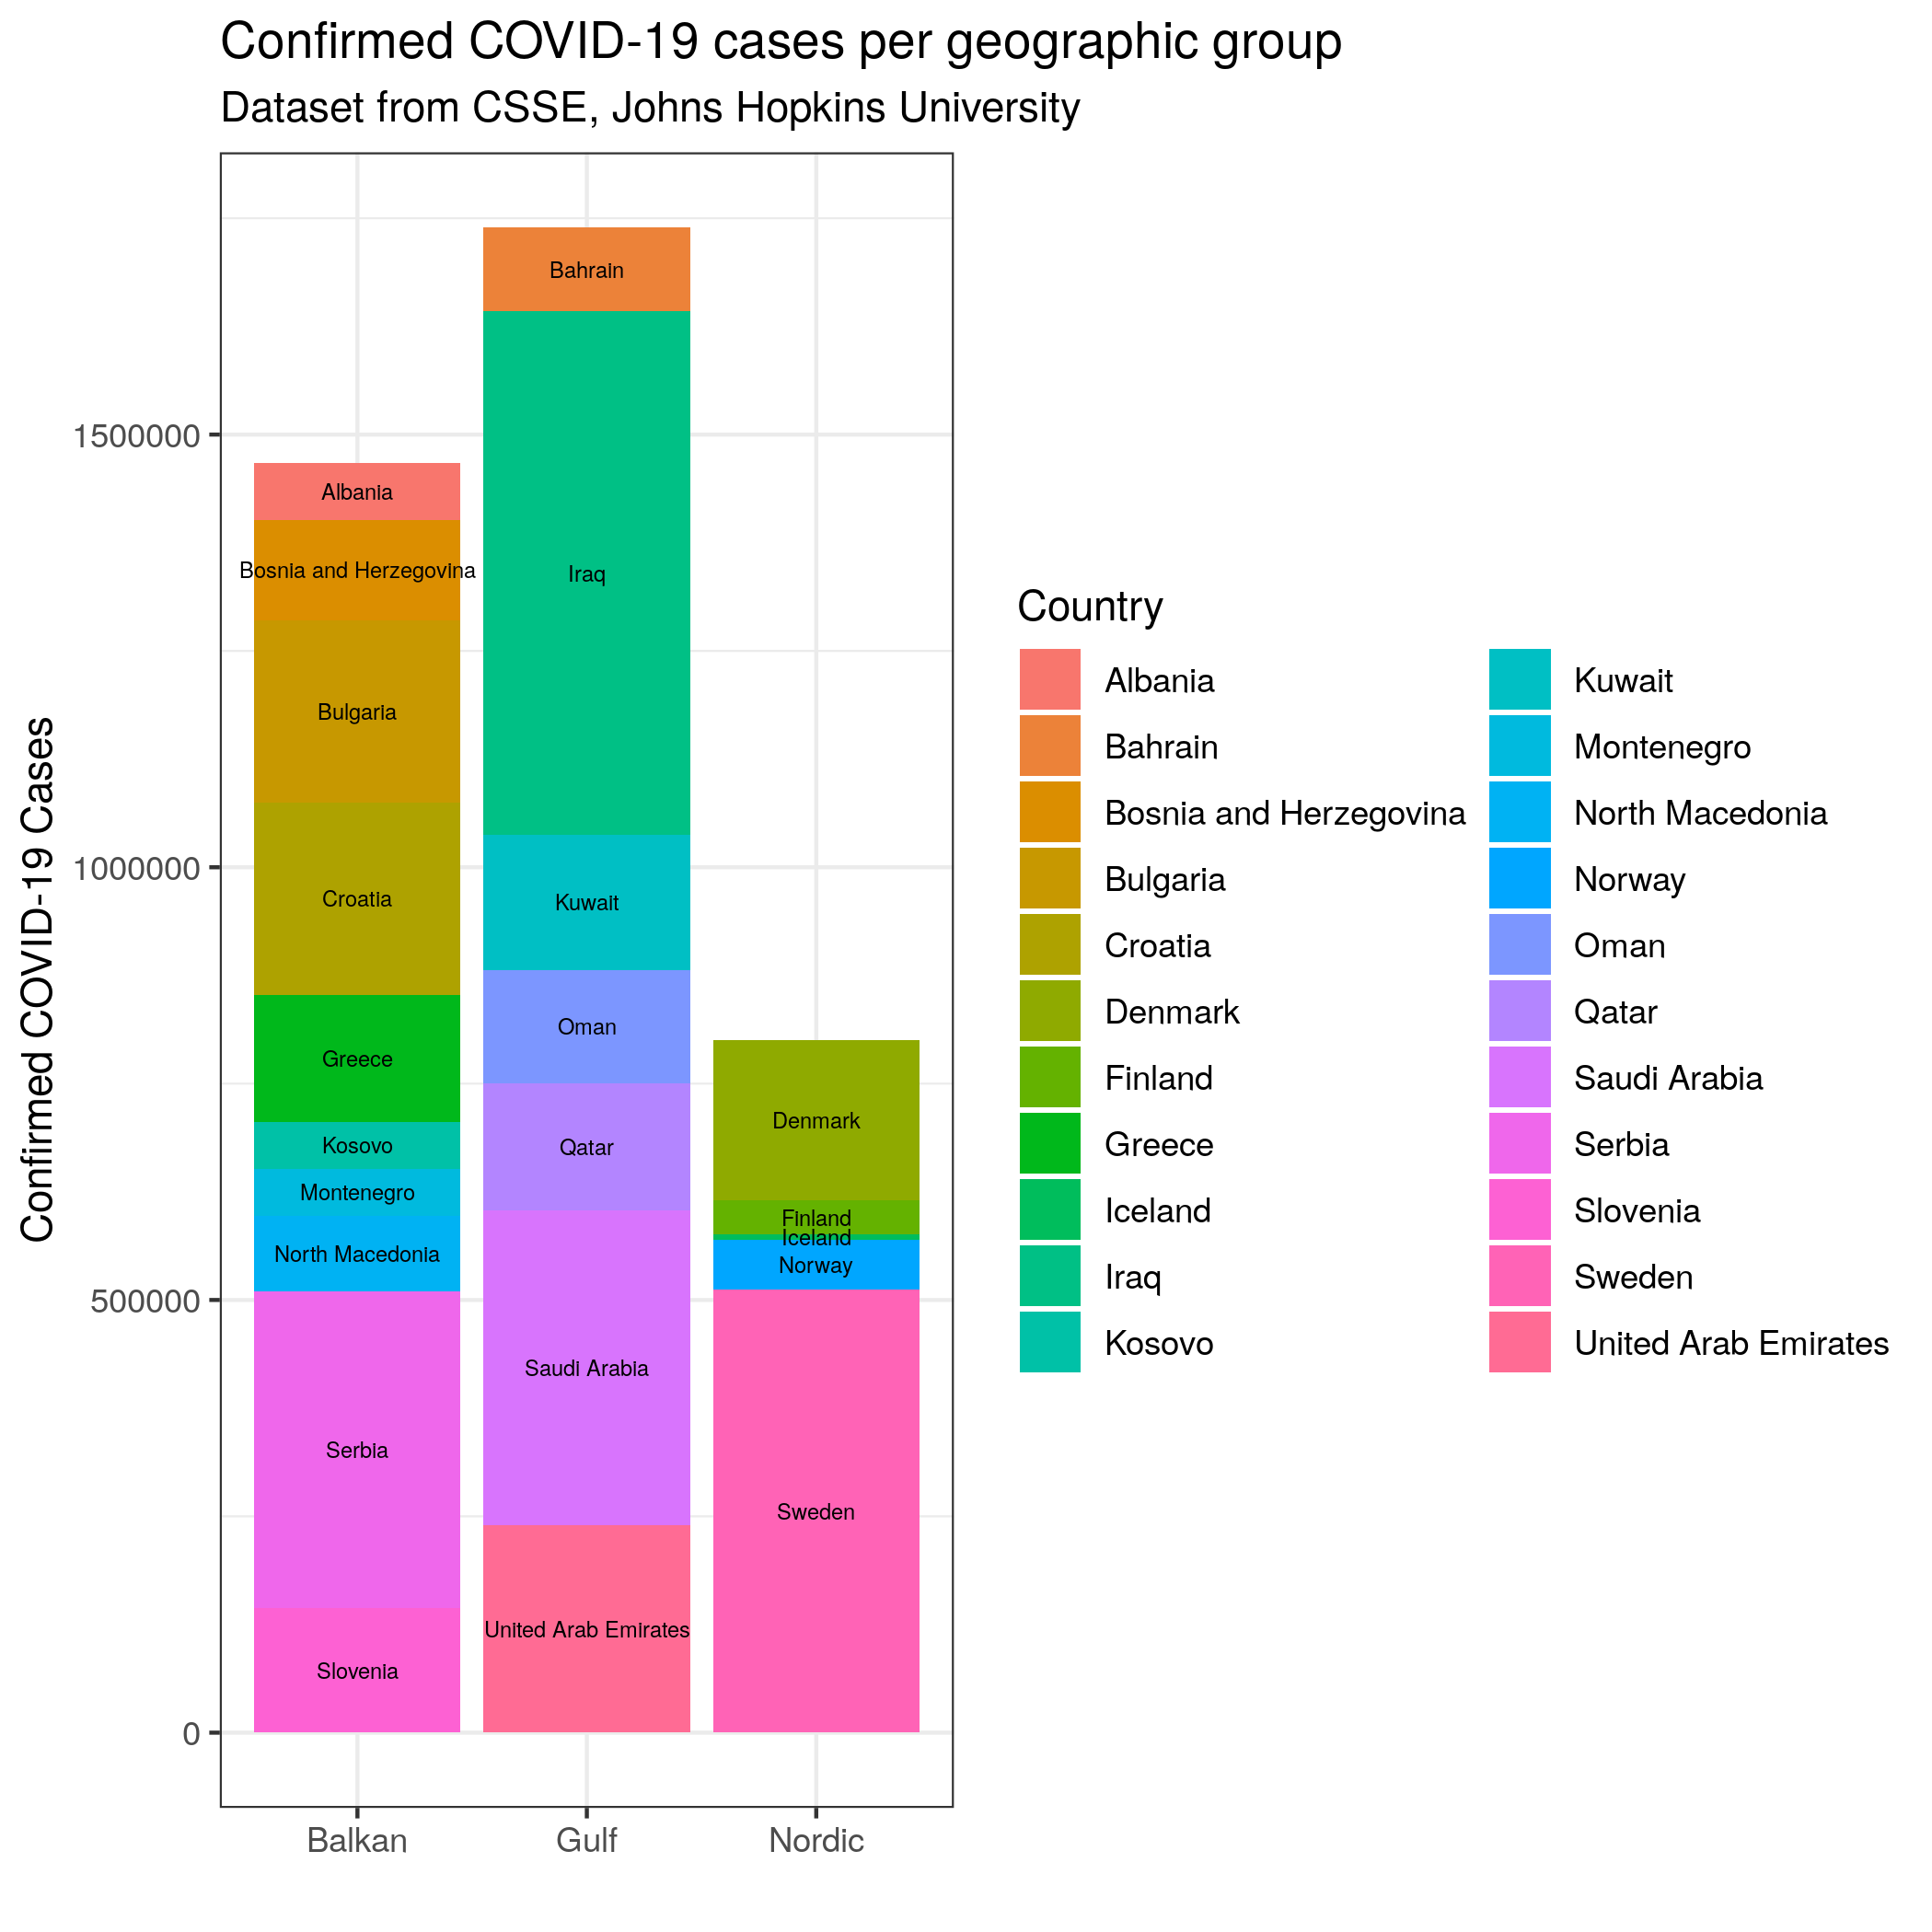
\includegraphics[width=1\linewidth]{images/aggr_geo_conf.png}
  \captionof{figure}{Confirmed COVID-19 cases per geographic group}
  \label{fig:aggr_geo_conf}
\end{minipage}%
\begin{minipage}{.5\textwidth}
  \centering
  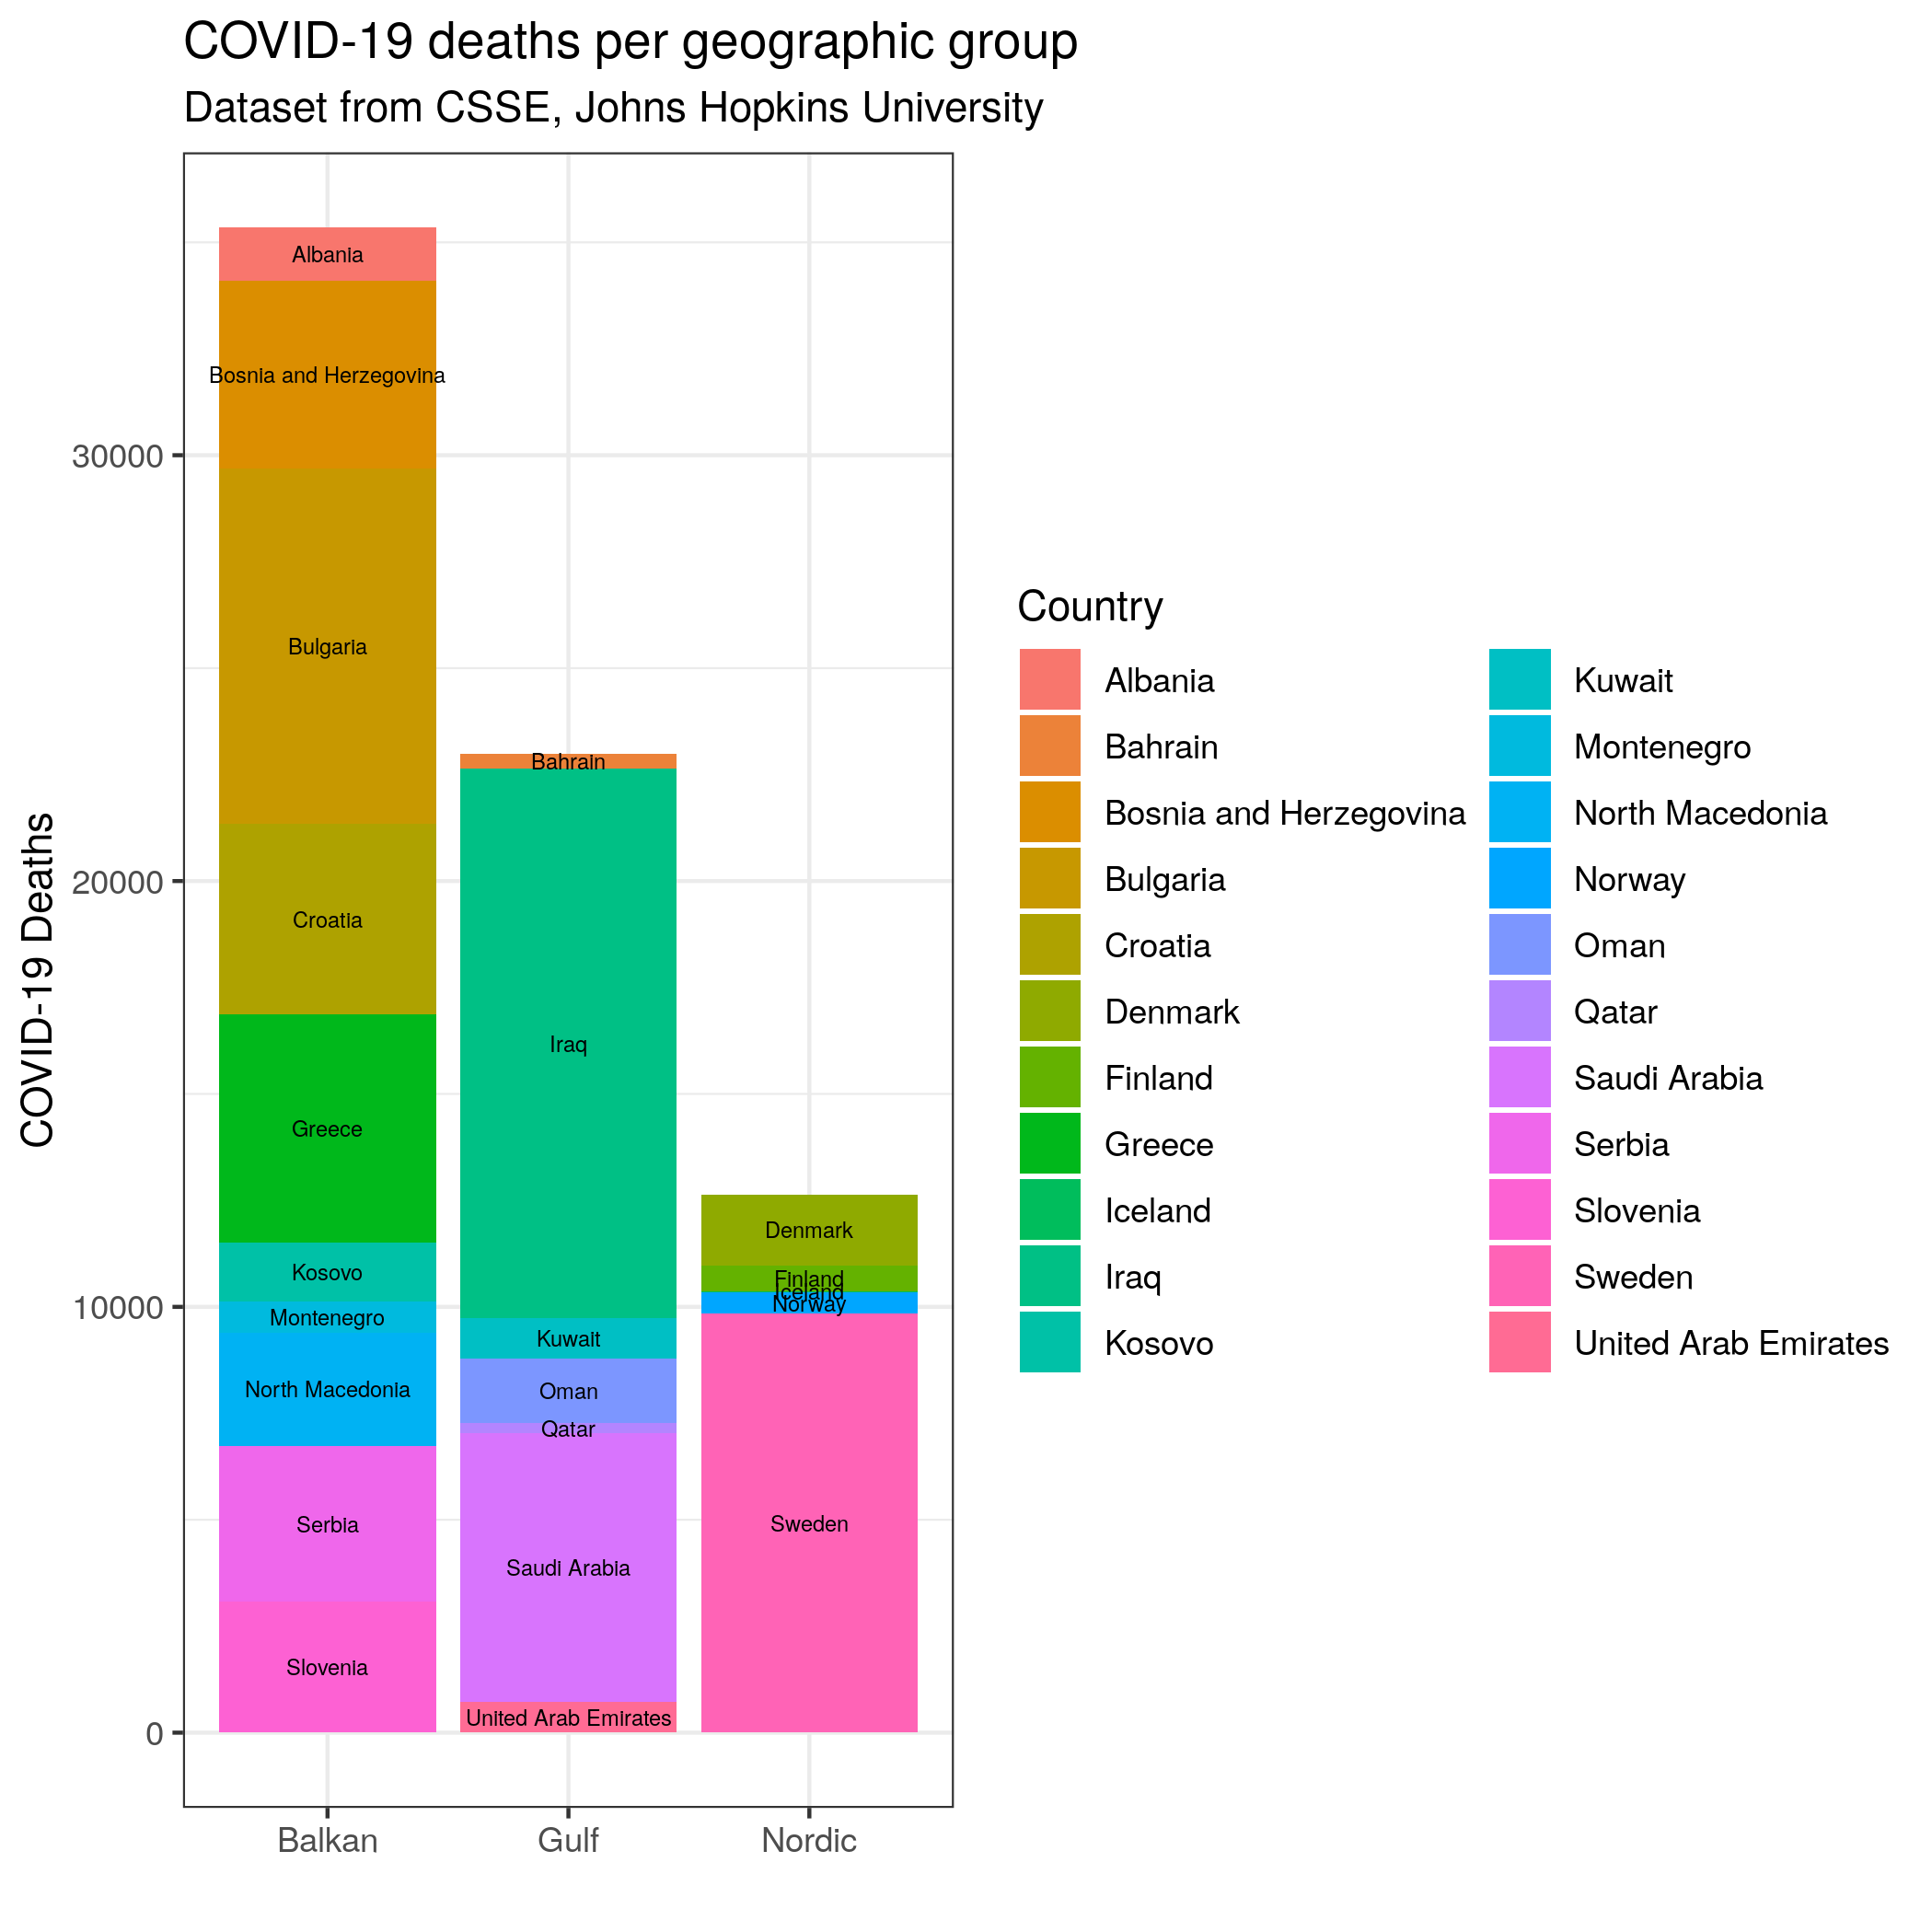
\includegraphics[width=1\linewidth]{images/aggr_geo_deaths.png}
  \captionof{figure}{COVID-19 deaths per geographic group}
  \label{fig:aggr_geo_deaths}
\end{minipage}
\end{figure}

\begin{figure}[H]
\centering
\begin{minipage}{.5\textwidth}
  \centering
  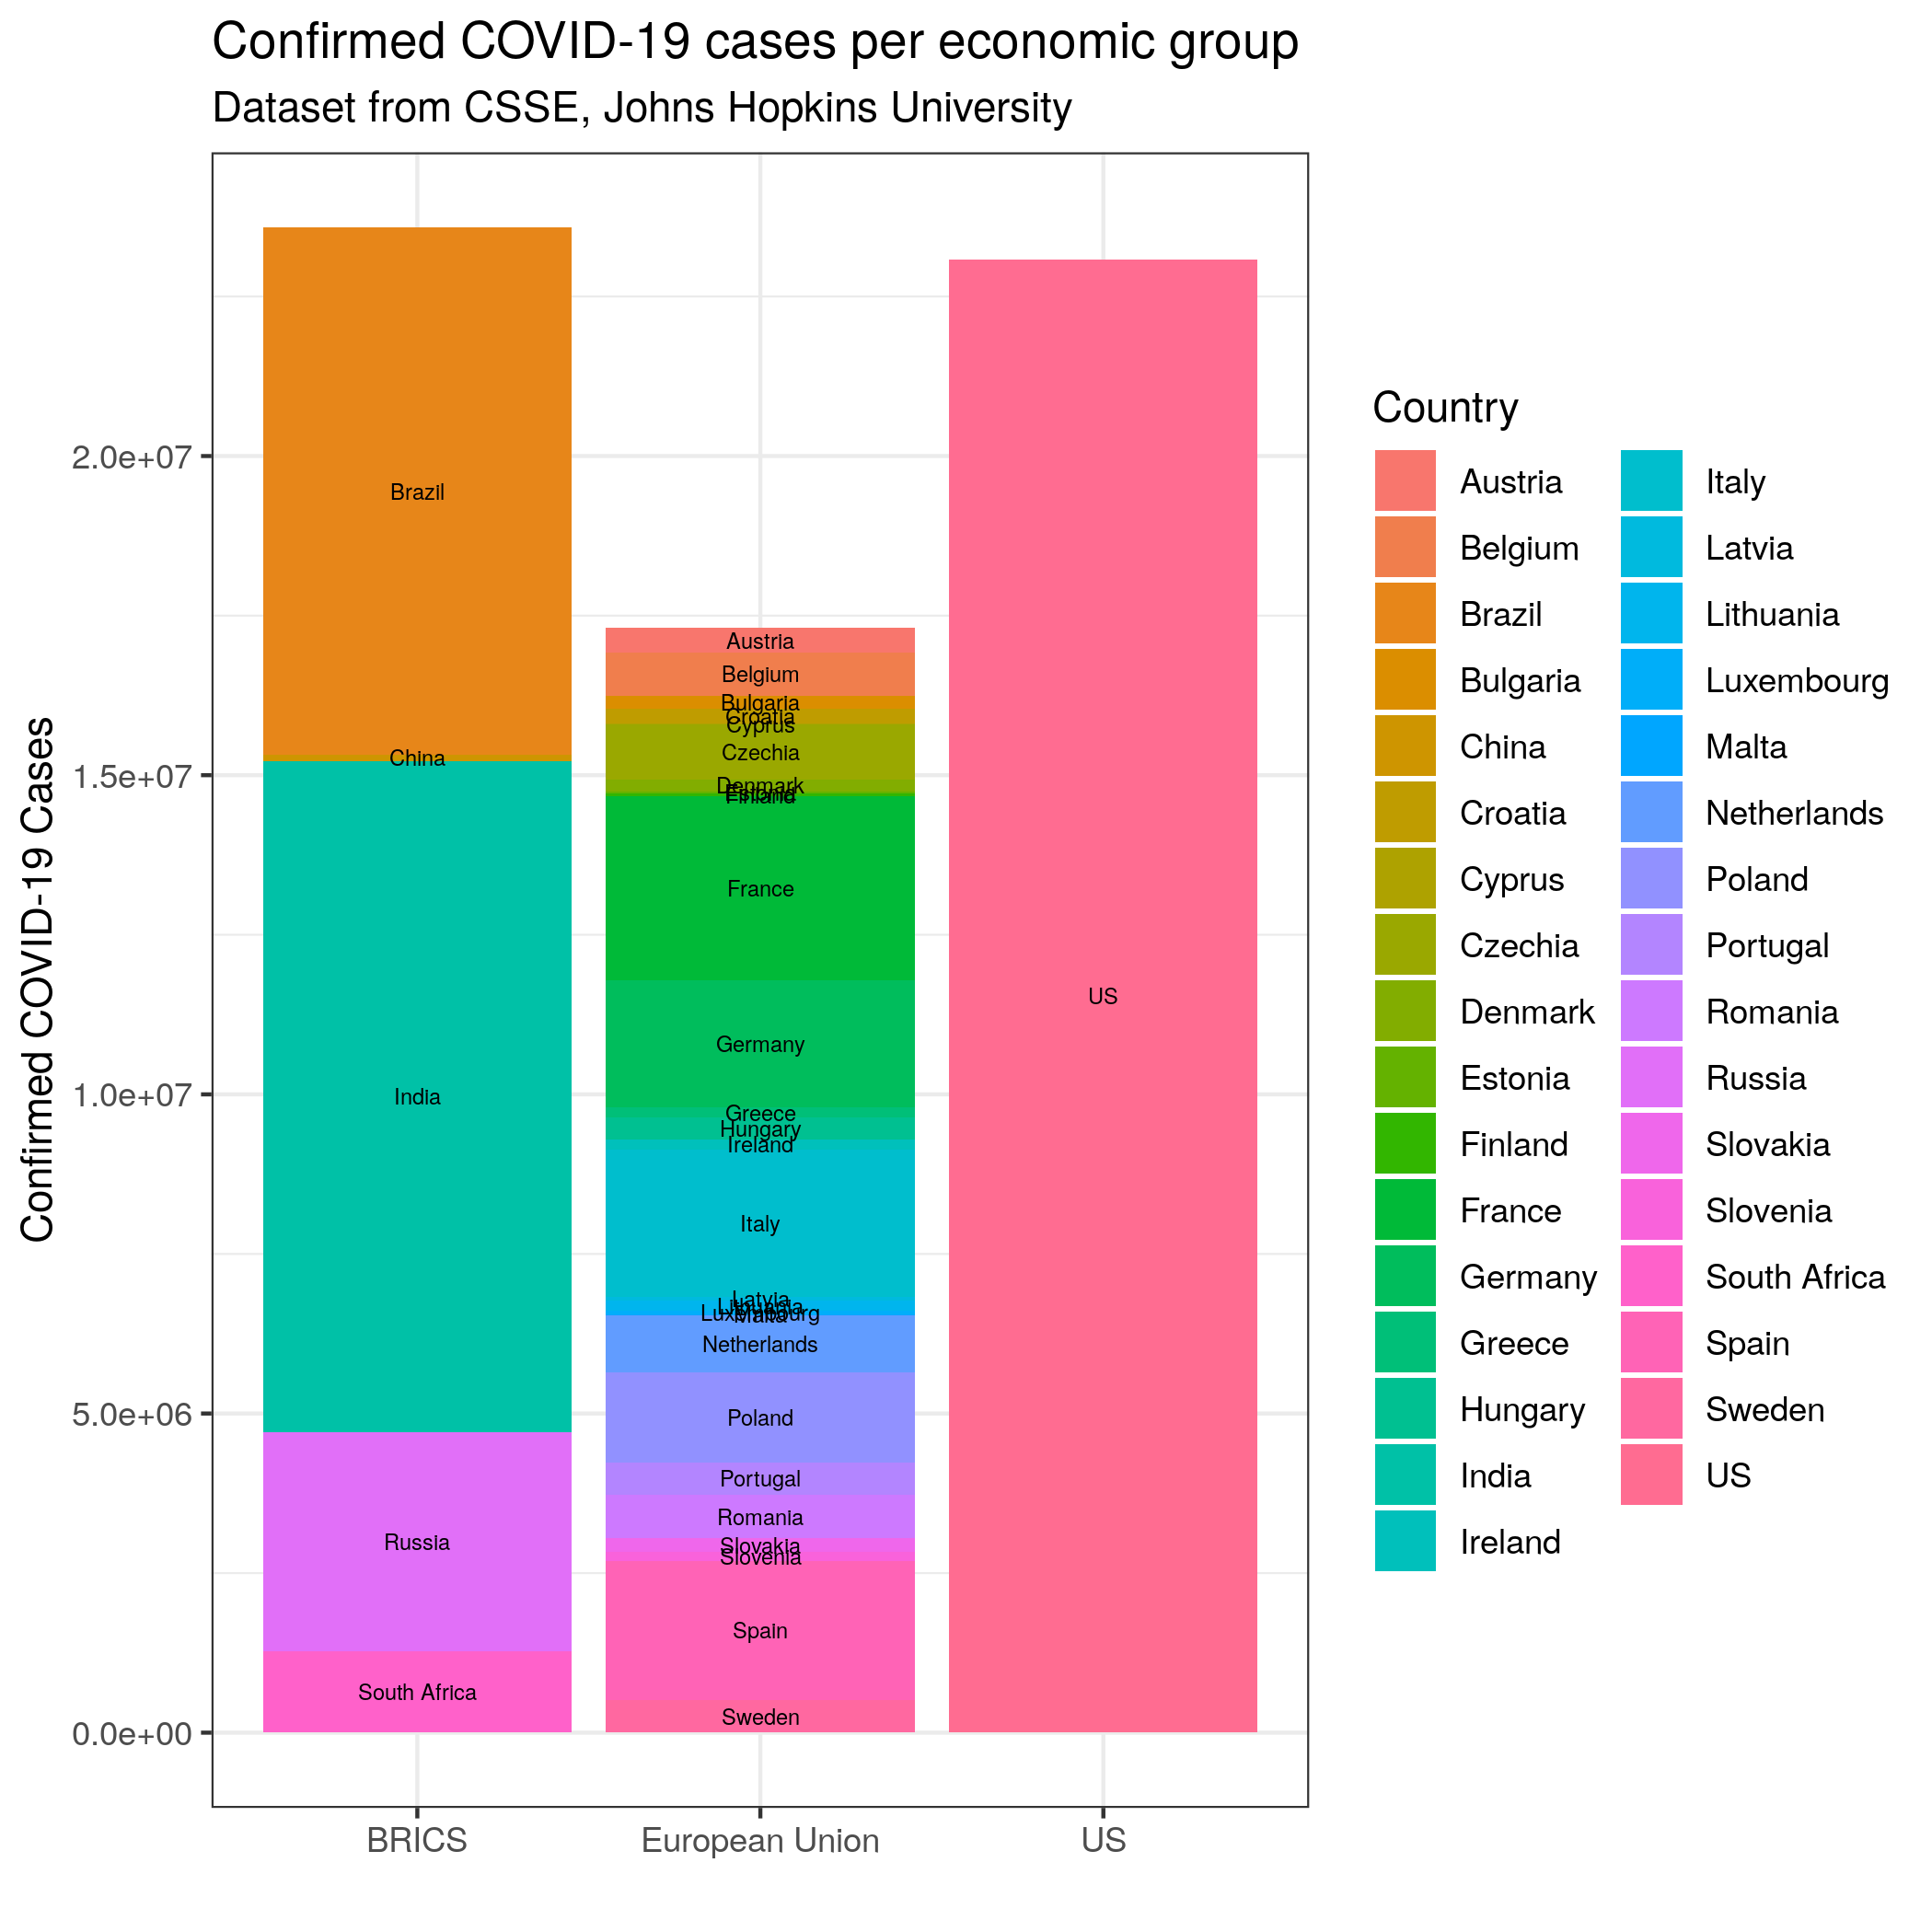
\includegraphics[width=1\linewidth]{images/aggr_econ_conf.png}
  \captionof{figure}{Confirmed COVID-19 cases per economic group}
  \label{fig:aggr_econ_conf}
\end{minipage}%
\begin{minipage}{.5\textwidth}
  \centering
  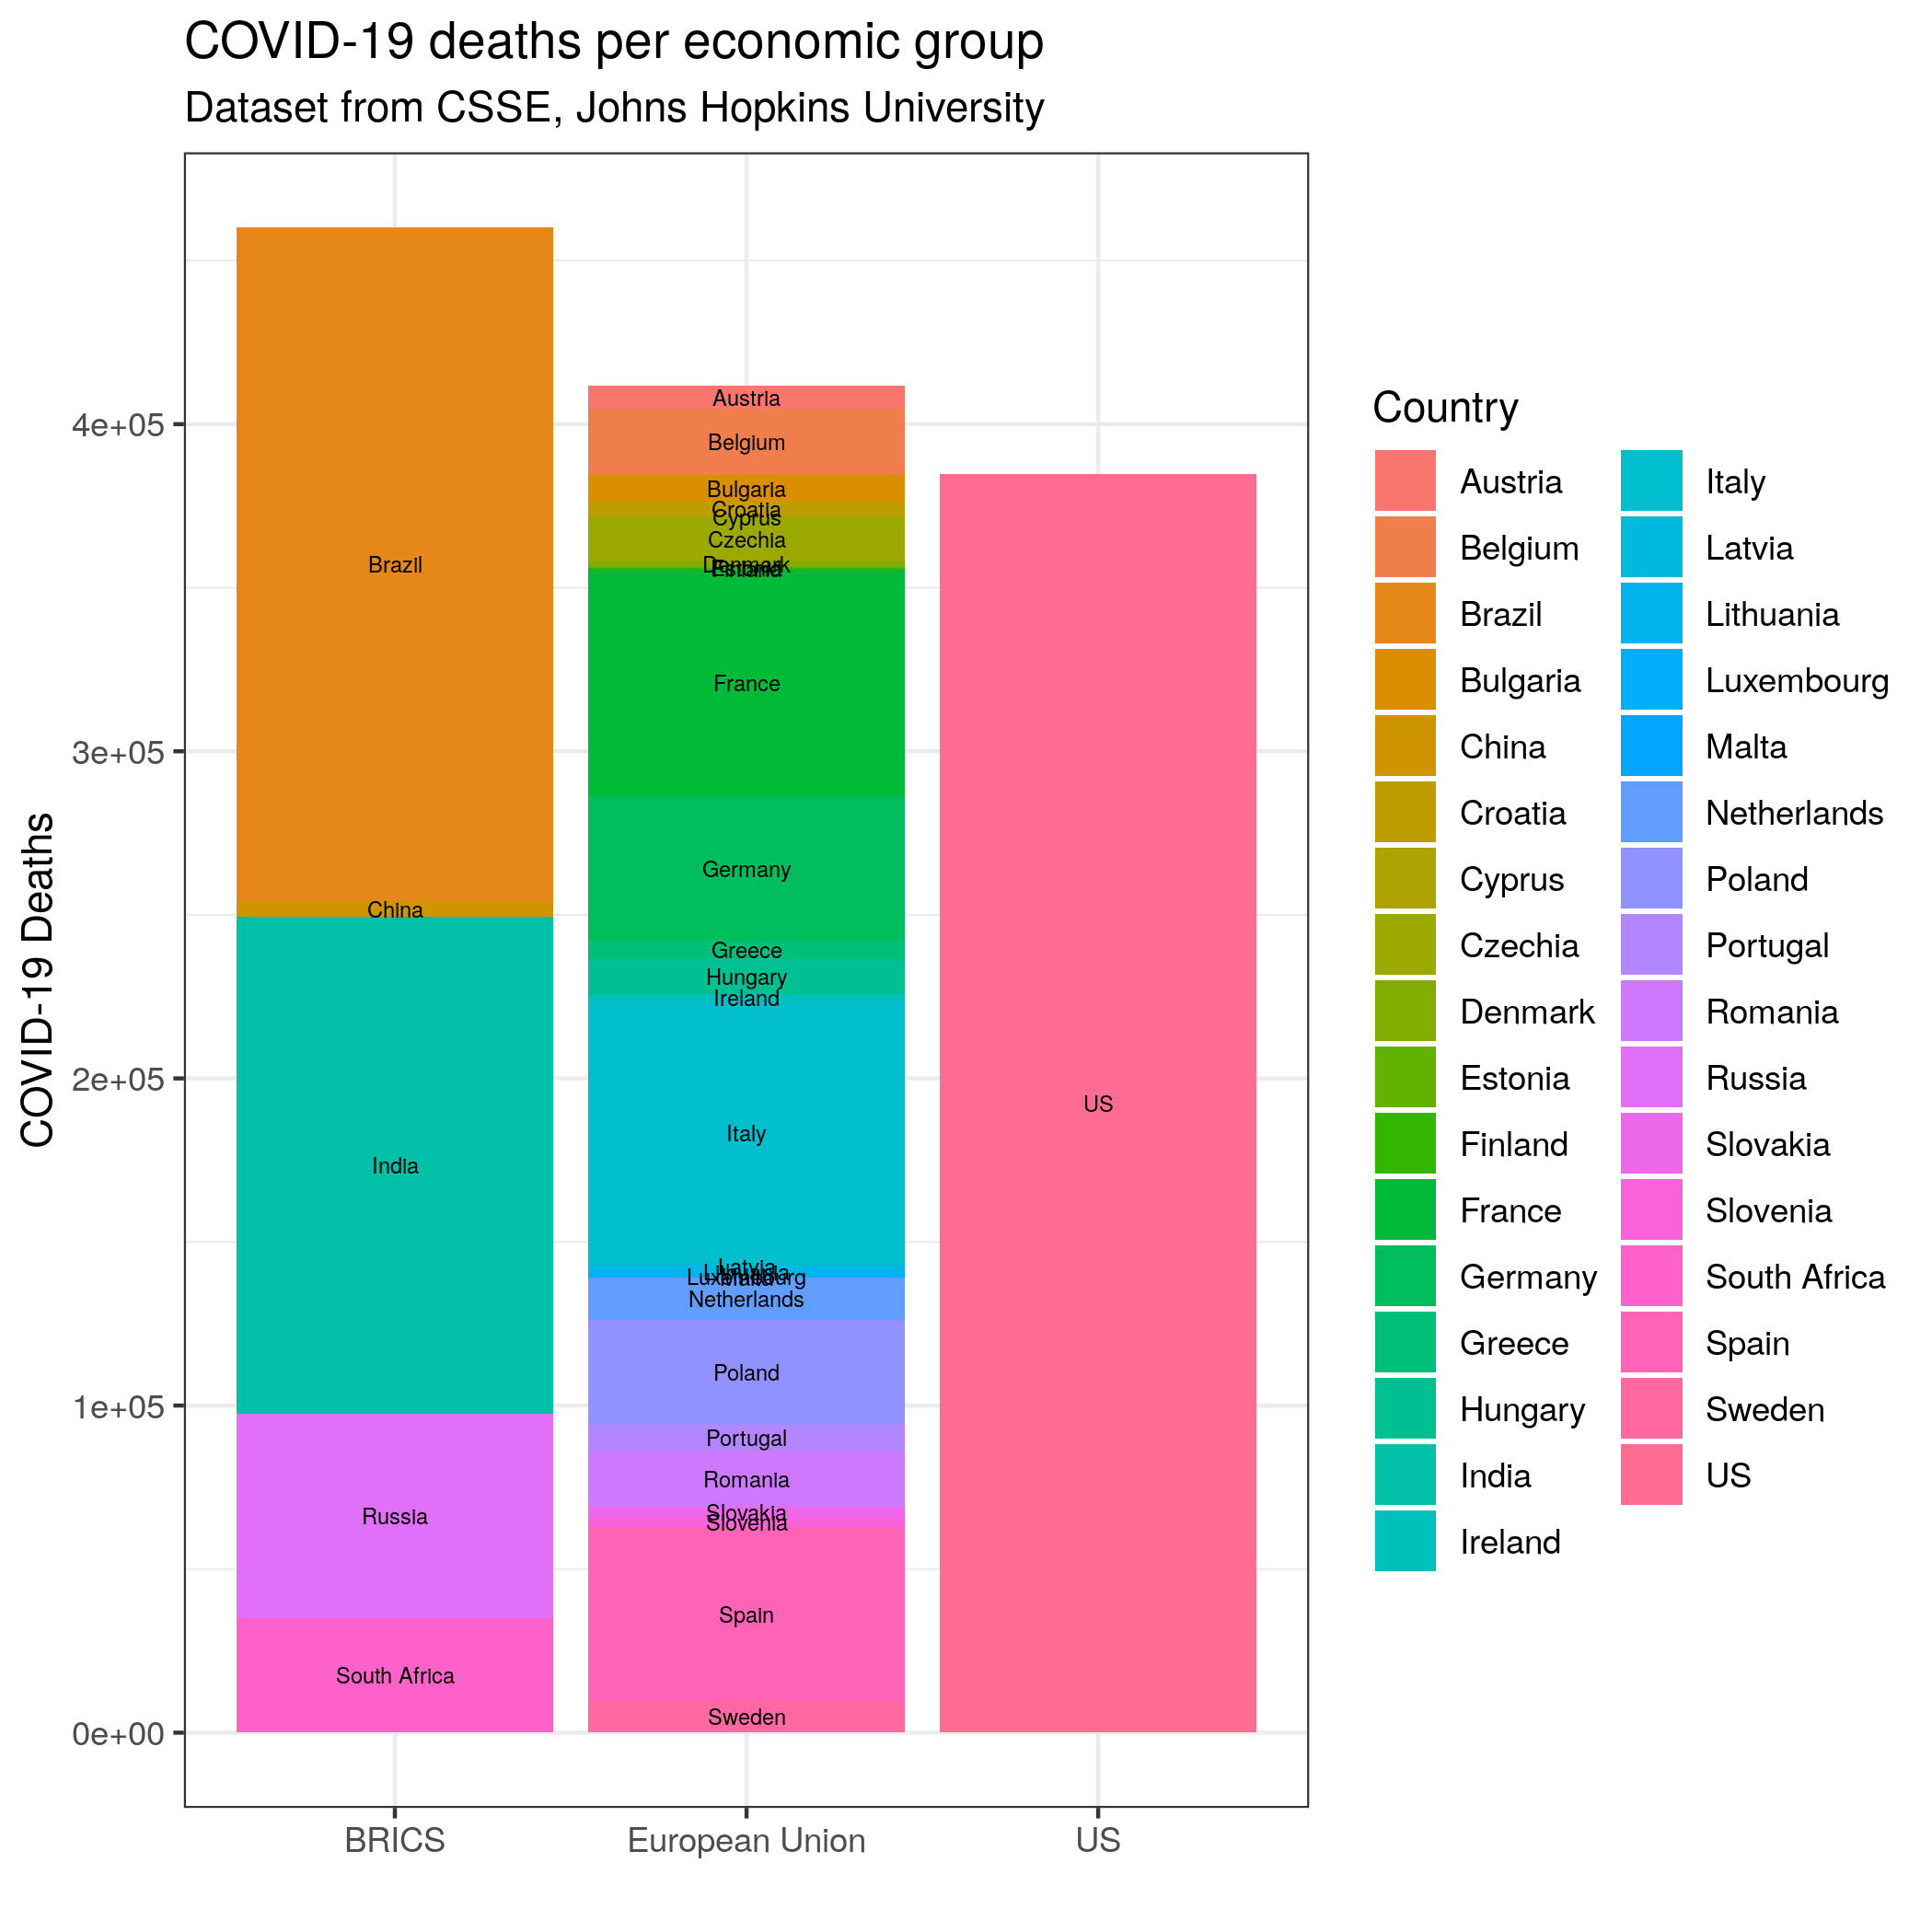
\includegraphics[width=1\linewidth]{images/aggr_econ_deaths.png}
  \captionof{figure}{COVID-19 deaths per economic group}
  \label{fig:aggr_econ_deaths}
\end{minipage}
\end{figure}

Finally, lines \ref{ratio_A}-\ref{ratio_Z} sort all countries (minus the reported cruise ships in the dataset) by their ratio of total COVID-19 confirmed cases to the total number of deaths attributed to the virus, and keep the worst $25$ of them.
These are merged with the joint stats of all previous groups of countries (both economic and geographic) and presented in Figure \ref{fig:aggr_lollipop}, each annotated with their actual number of deaths and confirmed COVID-19 cases.

\begin{figure}[H]
\centering
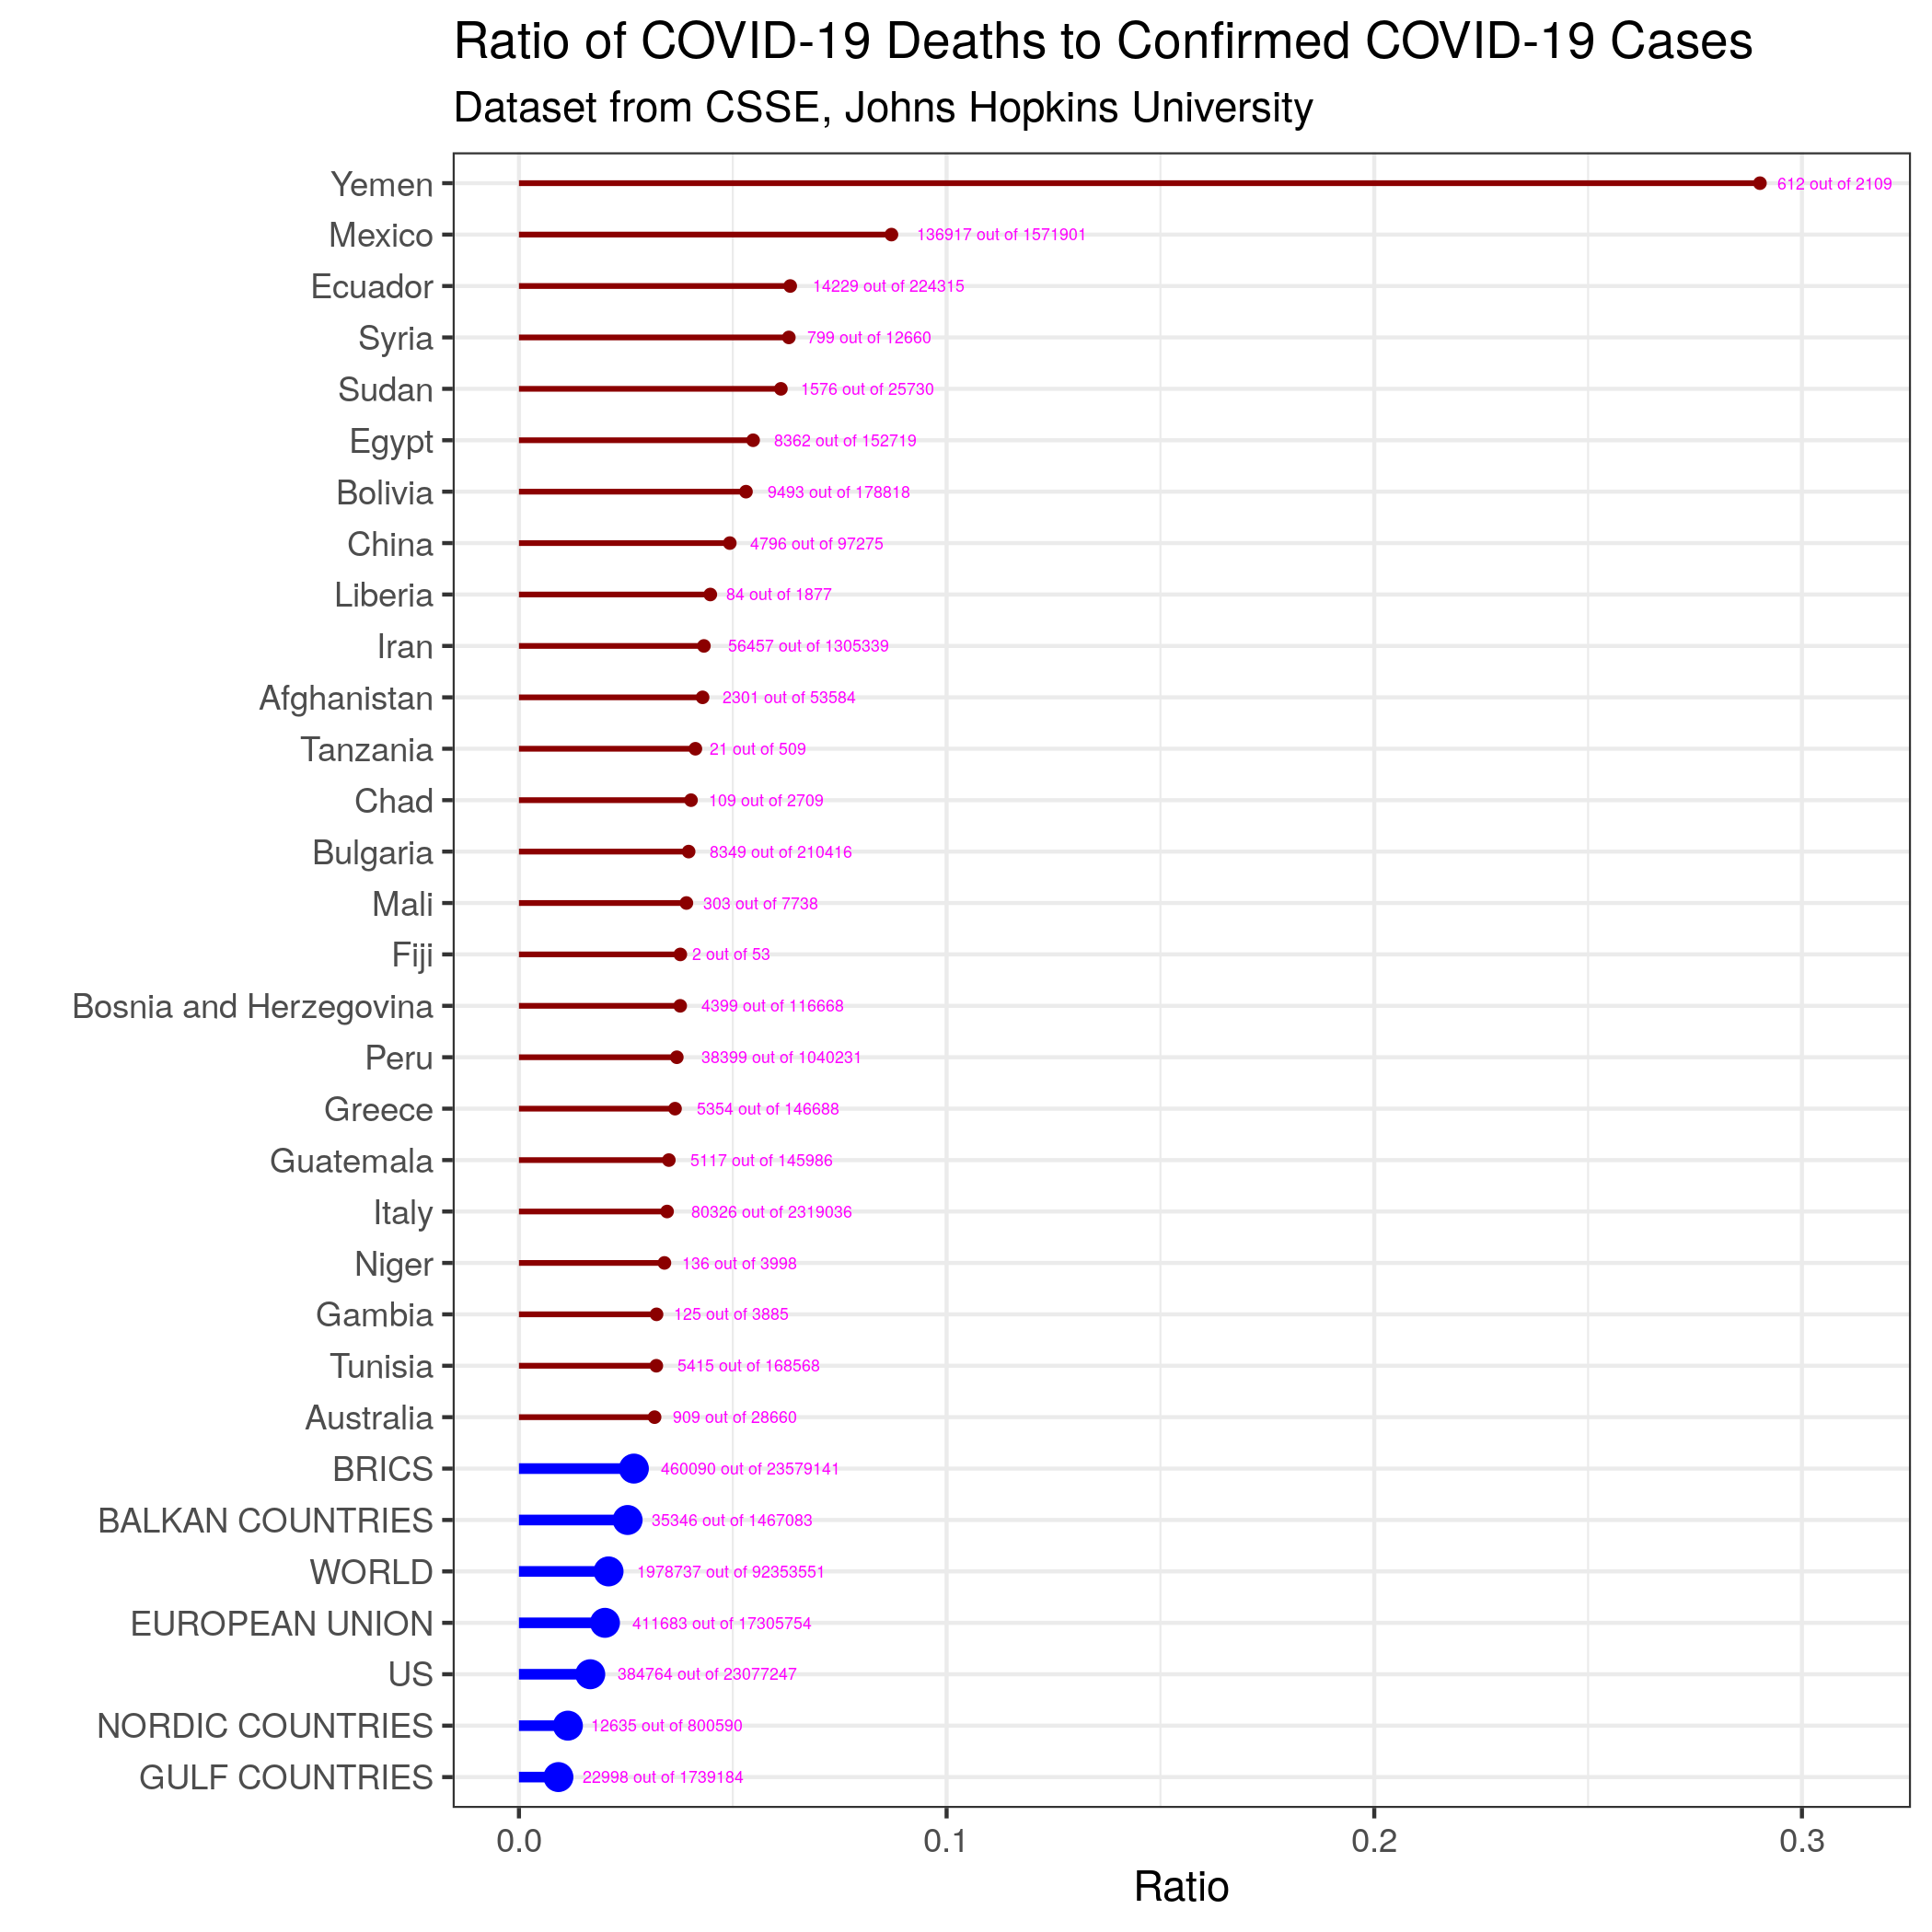
\includegraphics[width=1\linewidth]{images/aggr_ratio_lollipop.png}
\captionof{figure}{Ratio of COVID-19 Deaths to Confirmed COVID-19 Cases.}
\label{fig:aggr_lollipop}
\end{figure}

As it is made obvious by the diagram, countries that are either poor or isolated tend to have a higher ratio of deaths attributed to COVID-19 to confirmed cases of the virus, albeit larger countries, like Australia and Italy also appear in the bottom $25$ of them.
Sadly, Greece also appears in this list -- as a matter of fact it appears to be the third worst European country and the second worst within the European Union (after Bulgaria).
